\documentclass[main.tex]{subfiles}
\begin{document}
\section{Question 3}
Implement sleep using signal function which takes care of the following:
\begin{itemize}
  \item If the caller has already an alarm set, that alarm is not erased by the
    call to alarm inside sleep implementation.
  \item If sleep modifies the current disposition of SIGALRM, restore it
  \item Avoid race condition between first call to alarm and pause inside sleep
    implementation using setjmp.
\end{itemize}
Test the implementation of sleep by invoking it in various situations

\lstinputlisting[style=codeStyleC]{listings/3.c}
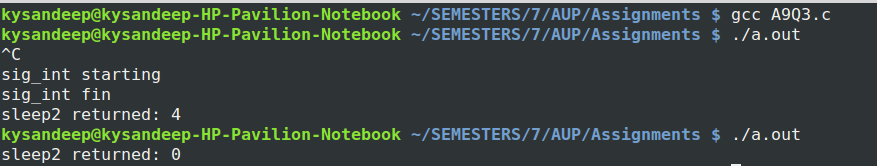
\includegraphics[width=\textwidth]{figures/3_output.png}
\end{document}
